\chapter{Real-time planlægning}
Vi vil i dette kapitel beskrive Real-time planlægning (RTP), samt diskutere hvordan det kan implementeres i \pycsp. 

RTP er baseret på den kendsgerning at nogle begivenheder i programmer kan være vigtigere at få udført end andre indenfor en afgrænset tidsperiode. Dette kan f.eks. være interrupts, input- eller output enheder eller interne processer. Med RTP tilknytter man en deadline for hver begivenhed, som bruges til at planlægge rækkefølgen for afvikling af begivenhederne. Formålet er at optimere antallet af begivenheder der når at blive udført inden deres deadline er overskredet. Normalt anses alle begivenheder for at være lige vigtige, og de planlægges ud fra en optimal udnyttelse af processoren. Denne optimale processorudnyttelse kan man være nødt til at gå på kompromis med hvis man ønsker at bruge RTP og derved prioritere visse begivenheder højere end andre. Man kan forestille sig en situation hvor man ikke starter en begivenhed med lav prioritet selv om den er klar, hvis man ved at en begivenhed med høj prioritet er klar kort tid efter, og venter derfor på at den er klar og igangsætter begivenheden med høj prioritet med det samme. 
RTP benyttes meget i specialiserede indlejrede systemer til f.eks medicinsk udstyr, kontrol af luftrummet, på rumstationen ISS\cite{Audsley1990} og mange andre steder. Det er dog også anvendeligt i i mere gængse applikationer, typisk i forbindelse med en eller anden form for interaktion med den virkelige verden. 

Indenfor RTP er der som udgangspunkt to kategorier af deadlines, henholdsvis soft og hard deadlines. Forskellen ligger i hvordan en deadline fortolkes, specielt med henblik på hvad der sker hvis en deadline overskrides. Hvis en soft deadline overskrides kan en færdiggørelse af begivenheden stadig bidrage med en positiv værdi til systemet, dog mindre end hvis deadlinen var blevet overholdt. Udførelse af begivenheder der har overskredet en hard deadline vil derimod ikke kunne bidrage positivt til systemet. For begge kategorier gælder det at en overskridelse af deadline i yderste konsekvens kan bidrage negativt til systemet. Nedenfor er gennemgået forskellige typer deadlines illustreret med time-value funktioner. Værdien er den enkelte begivenheds bidrag til programmets endelige mål. 

I \cref{fig:hard-dl} vises en hard deadline for en begivenhed. 

\begin{figure}
 \begin{center}
  
\includegraphics[scale=0.75]{images/hard-deadline}
	\caption{Begivenhed med hard deadline.}
	\label{fig:hard-dl}
\end{center}
\end{figure}
Her tilføres der en positiv værdi til programmet hvis begivenheden afsluttes mellem dens starttidspunkt og dens deadline. Hvis begivenheden først er færdig efter deadline har den ingen værdi. En soft deadline (\cref{figure:soft-dl}) tilføjer den samme værdi som en hard deadline hvis begivenheden bliver færdig rettidigt. 
\begin{figure}
 \begin{center}
  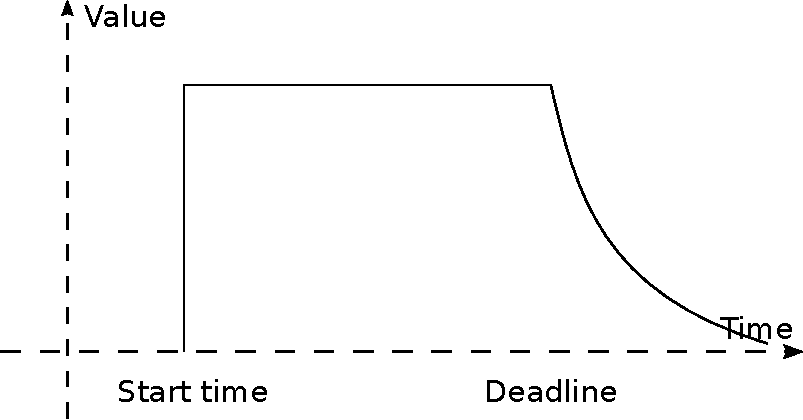
\includegraphics[scale=0.75]{images/soft-deadline}
	\caption{Begivenheden med soft deadline.}
	\label{figure:soft-dl}
\end{center}
\end{figure}
Hvis deadlinen overskrides mindskes værdien den begivenhed tilføjer, omvendt propotionalt med overskridelsen. Ved en hard deadline er der ikke tilknyttet en egentligt straf hvis en begivenhed ikke overholder sin deadline. Dette er derimod tilfældet i \cref{fig:hard-rtp}, der viser en begivenhed der tilføjer negativ værdi ved overtrædelse af en deadline. Hvis den tilknyttede straf for ikke at overholde en deadline er større end en hvad programmet maksimalt kan opnå ved at overholde alle deadlines kaldes det et ``hard real-time system''\cite{Laprie1989}.
\begin{figure}
 \begin{center}
  
\includegraphics[scale=0.75]{images/critical-deadline}
	\caption{Begivenhed med kritisk deadline.}
	\label{fig:hard-rtp}
\end{center}
\end{figure}

Generelt vil der i et real-time system ikke være alle begivenheder der har den samme type af deadline. Nogle begivenheder har ingen deadline, nogle har en soft deadline, og få har en hard deadline. For RTP skal kørslen planlægges så begivenhederne har den maksimale udnyttelse af tilgængelige ressourcer samtidigt med at så mange deadlines som muligt overholdes, hvor de vigtigte deadlines prioriteres højest. 

\section{Planlægning af begivenheder}
De fleste eksisterende real-time systemer arbejder på isolerede systemer, hvor planlæggeren har fuld kontrol over hele computeren. Derfor er hovedparten af forskningen indefor det praktiske område gået til udarbejdelsen af specialiserede kerner og komplette operativsystemer\cite{damm1989real, jones1979staros, levi1989maruti,ramamritham14scheduling}. Vi ønsker i modsætning hertil ikke at udvikle en specialiseret kerne, men lade \sched en i \pycsp kunne planlægge processer efter bedste evne baseret på informationer den har om processerne.

For real-time systemer kan begivenheder planlægges enten statisk eller dynamisk\cite{cheng1987scheduling}. I statisk RTP er alle begivenheder kendt på forhånd. Planlæggeren kan i dette tilfælde allerede inden start udregne om det er muligt at overholde alle deadlines. Alternativt planlægges begivenhederne dynamisk hvis der løbende kan ankomme nye begivenheder der skal planlægges. I realtidssystemer er næsten alle begivenheder cykliske, med enten en regelmæssig eller tilfældigt periode. Periodiske begivenheder kan være målinger der skal være foretaget med regemæssige intervaller, mens aperiodiske begivenheder kan forekomme som reaktion på udefra kommende begivenheder, eller være fejl, der hurtigt skal håndteres inden systemet kan fortsætte.
Til planlægningen har planlæggeren behov for at vide hvor lang tid det vil tage at udføre en given begivenhed per periode, men da dette tal enten ikke kan kendt eller fast for hver periode bruges der ofte estimater. Dette medfører at en aperiodisk begivenhed kan ankomme på et vilkårligt tidspunkt og da planlæggeren kun har et estimat for tidsforbruget kan man  ikke tilknytte en ``hard deadline'' til aperiodiske begivenheder, da der altid findes en kæde af aperiodiske begivenheder der medfører en overskridelse af en deadline. 

\fxnote*{Dette skal måske flyttes eller omformuleres så vi ikke med det samme begrænses til dynamiske \sched}{I \pycsp kan der til alle tidspunkter tilføjes nye processer, og derfor vil vi kun beskæftige os med en dynamisk \sched. Desuden har man ikke med \pycsp fuld kontrol over hele operativsystemet. Mængden af processerkraft vi har til rådighed til kørsel af processerne vil derfor varriere uafhængigt af \pycsp, hvorfor vi heller ikke kan lave et pålidelig ``hard real-time system'', men fokusere på et ``soft real-time system''.}

\subsection{Metoder til skemaplanlægning}
Der findes adskillige metoder til at planlægge rækkefølgen af begivenheder, alle med det formål at nå alle deadlines, og såfremt dette ikke kan lade sig gøre, så sikre at det er de mindst vigtige deadlines der overskrides. 

\begin{shaded}
Vi vil i dette afsnit fokusere på skemaplanlægning i et ``soft real time'' system, hvor processer ankommer dynamisk og diskutere fordele og ulemper ved dem.
To af de mest kendte \sched e til brug i real-time systemer er ``Rate monotonic algorithm''\cite{lehoczky1989rate,liu1973scheduling} og ``Earliest deadline first''\cite{liu1973scheduling}.


Hvor processer isoleret set har behov for at udføre deres opgave inden deres deadline, har \sched en behov for kvantitativt at kunne \fxnote*[inline,nomargin]{brugere sortere ?}{organisere} dem indbyrdes således den til hver tid kan vælge hvilken proces der næste gang skal udføres. Kernen i en  \sched ~ er derfor at gå fra en række processer med tilknyttet deadline og eventuelt andre egenskaber til en prioriteret liste 

De klassiske algoritimer behandler alle processer som værende ligeværdige. Vi har dog tidligere vist at processer kunne reagere forskelligt på en overskridelse af deres deadline. En \sched er stabil hvis man kan definere en mindre mængde processer som kritisk, og som deadline vil bliver overholdt selv hvis alle deadlines ikke kan overholdes.
\end{shaded}

\subsubsection{Rate monotonic algorithm (RM)}
RM er oprindeligt en statisk \sched, der fra start af udregner en prioritede liste på baggrund af frekvensen af processens periode, dermed vil processer der oftet skal have udført deres periode en højere prioritet, end processer med lav frekvens. RM er todelt og i første del udføres før selve simuleringen udregnes  prioriteten for processerne, og udvælger hvilke processer der kan medtages i selve udførslen. Anden del står for udvælgelsen af processer  under simuleringen, og her vælges simpelt den proces med den højeste prioritet. 

 Et problem for RM er at ved udvælgelsen af processer der kan medtages har man ikke en optimal udnyttelsen af processorkraf. \Citeauthor{lehoczky1989rate} er kommet frem til at ``worst-case'' er udnyttelsen i gennemsnit 88\\cite{lehoczky1989rate}. Et større problem i relation til implementering i \pycsp er dog at RM er dog at den er statisk. Til gengæld er algoritmen stabil ved en overskridelse af deadline for en proces. 

\subsubsection{Earliest deadline first (EDF)}
Som alternativ til den statiske \sched, hvor man ikke kan ændre prioriten af processen løbende gennem simuleringe, findes de dynamiske \sched er, hvor er EDF er et eksempel. Her evalueres prioriterne af processerne dynamisk igennem simuleringen og evaluere dermed løbende hvilke processer der skal udvælges. I EDF har den proces hvis deadline ligger tættest på højest prioritet og den hvis proces har længst til deadline den laveste prioritet. Aperiodiske processer kan i EDF indgå på lige fod med de periodiske da man til hvert processkift evaluere hvilken der har den nærmeste deadline, som både kan være en periodisk proces som en aperiodisk.

Udnyttelsen af processorkraft kan i EDF komme op på 100\, da alle processer bliver planlagt løbende i modsætning til RM der foretager et valg om en given proces kan planlægges.  Ulempen ved EDF er den ikke er stabil i det vi ikke har kontrol over hvilke processers deadline der bliver overskredet. Dette er specielt et problem hvis man har en en uhomogen samling processer hvor en mindre del er kritiske.

\subsubsection{Least Laxity(LL)}
LL er en modifikation af EDF. LL kigger på hvor lang tid en begivenhed tager at udføre sammenholdt med hvor lang tid der er til deadline for begivenheden. Laxity er defineret som deadline minus tiden det tager for at udføre begivenheden. Laxity bliver altså et udtryk for hvor presserende det er at igangsætte en begivenhed for at den kan nå sin deadline. I LL bruges dette til at prioritere de begivenheder der har mindst laxity højest når begivenhederne planlægges. 

\subsection{Blokkerede processer}
I den teoretiske tilgang til RTP antages det ofter at processerne er periodiske, har en fast eksekverings tid per periode og er uafhængig af andre processer, og køres i et isoleret miljø. De forskellige tilgange til RTP fokusere på hvordan man kan overvinde de enkelte antagelser ved isoleret og ophæve en af begrænsningerne.

Dette er en højst idealiseret verden og i en introduktion af RTP i PyCSP vil processerne ikke overholde et eneste af disse antagelser. 
I \pycsp bruges rendezvous til at blokerer kommunikerende  processer.

Vi vil nu beskrive problemerne ved at processerne er afhængige af hinanden, og kan blokere hinanden, således at en proces med høj prioritet venter på processer med lavere prioritet. Forestil dig i \pycsp tre processer ($P_0,P_1,P_2$)med prioriteterne $Pr_0>Pr_1>Pr_2$. Først udvælges $P_0$ da denne har højst prioritet, men stopper da den skal kommunikere med $P_2$. Den næste proces der udvælges vil være $P_1$, og dermed bliver $P_0$ unødigt forsinket mens $P_1$ kører. Dette kaldes priority inversion\cite{sha1990priority}.

Der findes overordnet set to metoder til at løse problemet med priority inversion. Enten kan man ungå at blokerer processer, eller man kan benytte priority inherience\cite{sha1990priority}. Med \pycsp kan man ikke ungå at processer kommunikere, og dermed vil kunne blokere hvorfor priority inherience er den enste farbare vej hvis man skal sikre optimal planlægning.

\subsection{Priotetsnedarvning}
Skelne mellem read og write
måske skal en kanal arve prioritet?
hvornår skal prioriteten ændres? 

2 cases:
udvælgelse i alternation
propagering af prioritet

med nedarvning kan en proces uden deadline arve en høj prioritet uden at få sat en deadline. 

Skal processer der arver prioritet også arve deadline? Det skal de nok ikke, da de så kommer til at kaste exceptions selv på deadlines som brugeren ikke har sat. De skal nok kastes af den oprindelige proces med information om hvad den ventede på da den fejlede. 

  \section{Eksempel}
  \section{Design og implementation}
  \section{Evaluering}
  \section{Fremtidigt arbejde}
  \section{Opsummering}
